\section*{Introduction}
This report describes the implementation and results of a rasterization algorithm applied to a wel-known 3D model. The algorithm uses a pinhole camera and supports direct illumination with camera rotation and translation, 

\setcounter{section}{1} 

\section{Drawing vertices}

Vertices of the 3D model are projected on the screen according to the following formula with $R$ the rotation matrix describing the camera direction, $C$ the camera position, $P$ the 3D coordinates of the vertex and $P'$ the 2D coordinates of the pixel on the screen.
\begin{equation}
P' = (P - C) * R
\end{equation}

Vertices x and y coordinates are then updated according to the pinhole camera model in order to obtain a perspective projection ($f$ focal length):
\begin{equation}
\begin{split}
x = f \frac{x}{z} + \frac{width}{2}\\
x = f \frac{y}{z} + \frac{height}{2}
\end{split}
\end{equation}

\begin{figure}[H]
\centering
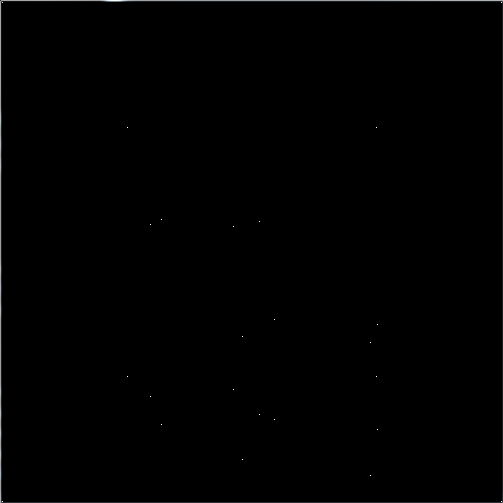
\includegraphics[width=0.4\linewidth]{img/points.jpg}
\caption{Triangles vertices projected by a pinhole camera}
\end{figure}


\section{Drawing edges}

Once the 2D position of the vertices is computed, we interpolate the 2D position of each point of the edges.

The camera translation and rotation using the arrow keys or the mouse has also been implemented. Rotation is however only applied to the Y axis.

\begin{figure}[H]
\centering
\minipage[t]{0.4\textwidth}
    \centering
    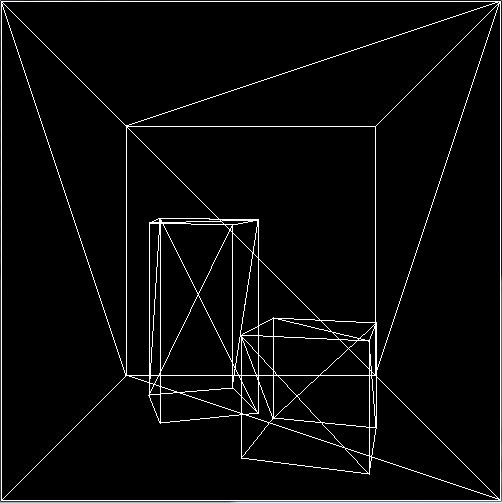
\includegraphics[width=\linewidth]{img/edges1.jpg}
    \caption{Triangles edges}
\endminipage
\minipage[t]{0.4\textwidth}
    \centering
    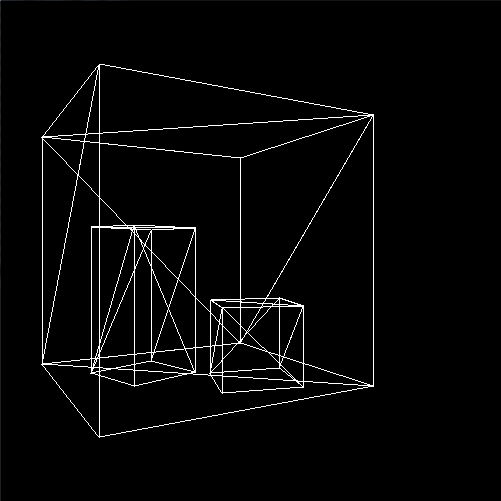
\includegraphics[width=\linewidth]{img/edges2.jpg}
    \caption{Triangles edges with camera rotation and translation)}
\endminipage
\end{figure}

Due to the current absence of clipping process in this algorithm, undesirable visual effects (figure \ref{fig:bug1}) may appear when rotating the camera of $90 \degree$. Those effects come with higher computation time.

Figure \ref{fig:bug2} shows a previous bug which happened for a rotation of $180 \degree$ and was caused by pixels displayed with coordinates out of range.

\begin{figure}[H]
\centering
\minipage[t]{0.4\textwidth}
    \centering
    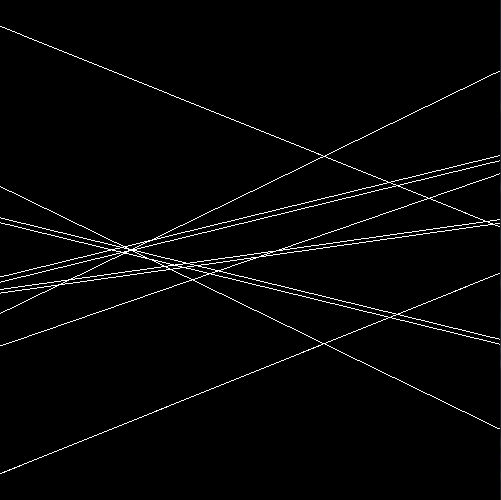
\includegraphics[width=\linewidth]{img/bug1.jpg}
    \caption{Bug sample - Camera rotation on the Y axis of $90 \degree$}
    \label{fig:bug1}
\endminipage
\minipage[t]{0.4\textwidth}
    \centering
    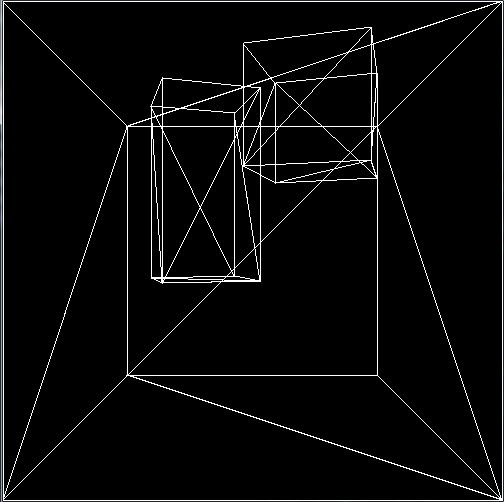
\includegraphics[width=\linewidth]{img/bug2.jpg}
    \caption{Previous bug sample - Camera rotation on the Y axis of $180 \degree$}
    \label{fig:bug2}
\endminipage
\end{figure}


\section{Filling triangles}

In order to fill triangles, the rasterization algorithm computes rows of pixels describing a given triangle.

A row is an array of pixels positions interpolated from the row boundaries. Those boundaries have the same Y coordinate but different X coordinates.

The boundaries are obtained by looping through the pixels of the edges in order to retrieve the minimum and maximum X for a given Y in the specified triangle.

By interpolating the pixels positions between the boundaries in each row, we eventually display every pixel of a triangle according to the triangle color.

Figure \ref{fig:colors} shows a rendering of the algorithm, computed in 8 ms. For a comparison, a similar rendering was obtained with the raytracer in 370 ms. We can observe that the blue box is displayed on top of the red box. This issue should be solve in the next section using a depth buffer.

Figure \ref{fig:colors_bug} is a previous bug sample obtained when rotating the camera and caused by invalid pixels positions when triangles vertices were out of the field of view.

\begin{figure}[H]
\centering
\minipage[t]{0.4\textwidth}
    \centering
    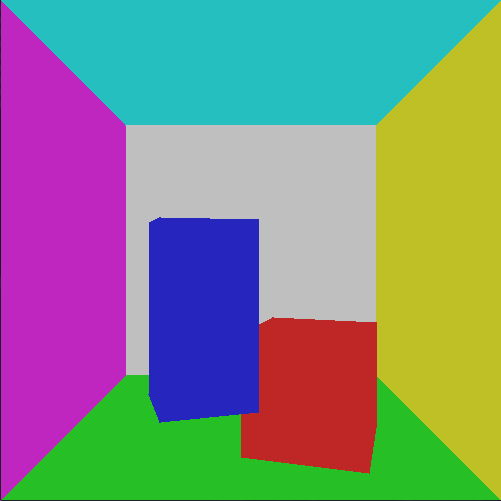
\includegraphics[width=\linewidth]{img/colors.jpg}
    \caption{Filled triangles}
    \label{fig:colors}
\endminipage
\minipage[t]{0.4\textwidth}
    \centering
    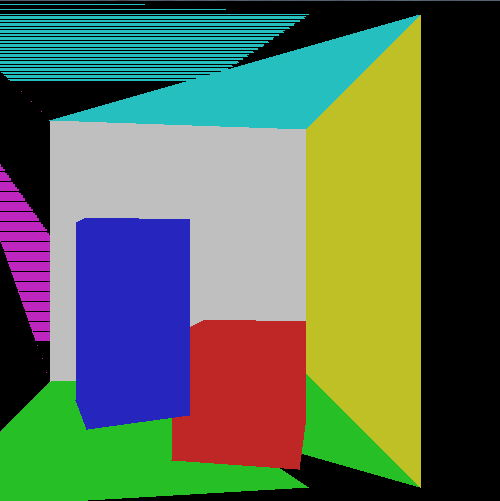
\includegraphics[width=\linewidth]{img/colors_bug.jpg}
    \caption{Previous bug sample}
    \label{fig:colors_bug}
\endminipage
\end{figure}


\section{Depth buffer}

The depth buffer is a structure containing the depth of each pixel displayed on the screen. When computing a new pixel, the rasterization algorithm should draw the corresponding pixel only if this one is closer to the camera than the on currently displayed.

This could be achieved by storing the interpolated Z coordinate of each pixel displayed in the depth buffer. However, due to the perpective projection applied by the pinhole camera model, this coordinate does not vary linearly. This is why we use here $\frac{1}{Z}$ instead, and display a new pixel when its $\frac{1}{Z}$ coordinate is larger.

In order to retrieve the initial Z coordinate, we could simply divide a linearly interpolated Z coordinate by $\frac{1}{Z}$. This value will be used in section \ref{subsec:perpixel}.

\begin{figure}[H]
\centering
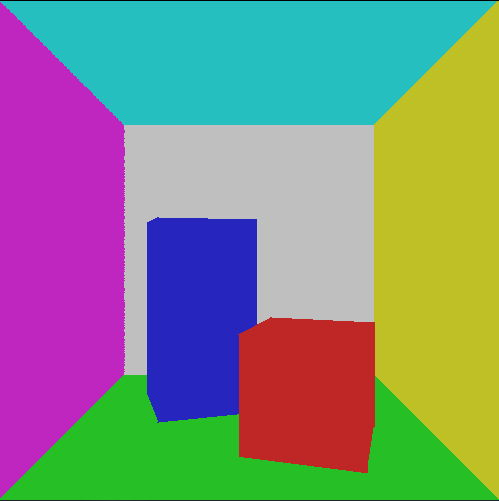
\includegraphics[width=0.4\linewidth]{img/depth_buffer.jpg}
\caption{Filled triangles with depth buffer}
\end{figure}



\section{Illumination}
\subsection{Per vertex - Interpolated light}
An illumination method giving speed renderings but poor realism (especially with large triangles) is to compute the illumination of every vertex and then to interpolate the illumination of the pixels inside the triangles.

The illumination model, same as the direct light model in the raytracer, is as follows, with \textit{D} the light power at the vertex, \textit{P} the power of the light source, i.e. energy per time unit for each color component (14.f * vec3( 1, 1, 1 ) for example), r the distance from the vertex to the light source, $\hat{n}$ the normal of the triangle and $\hat{r}$ a unit vector describing the direction from the vertex to the light source.

\begin{equation}
\label{eq:power}
D = \frac{P * max(\hat{r} . \hat{n}, 0)}{4 \pi r^2}
\end{equation}

The color of a vertex is then computed according to \textit{N} the indirect illumination constant and $\rho$ the RGB vector of a triangle.

\begin{equation}
R = \rho * (D+N)
\end{equation}

Once the vertices illumination \textit{R} is computed, we interpolate it for the pixels of the triangles edges, and then for the pixels of each row.

The rendering displayed in figure \ref{fig:interpolated_light} is computed in 14 ms.

\begin{figure}[H]
\centering
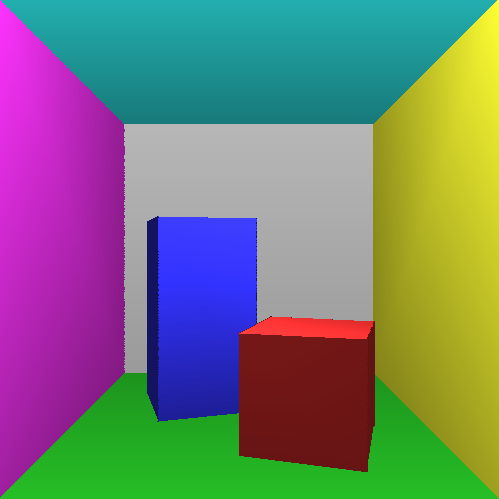
\includegraphics[width=0.4\linewidth]{img/interpolated_light.jpg}
\caption{Illumination with interpolated light}
\label{fig:interpolated_light}
\end{figure}

\subsection{Per pixel - Interpolated positions}
\label{subsec:perpixel}

Finally and to make our rendering more realistic, we apply the illumination model to every pixel instead of every triangles vertices.

To do so, we interpolate the 3D position of the pixels in addition to their 2D position. Nevertheless, interpolating the Z coordinate linearly gives the renderings below.

\begin{figure}[H]
\minipage[t]{0.33\textwidth}
    \centering
    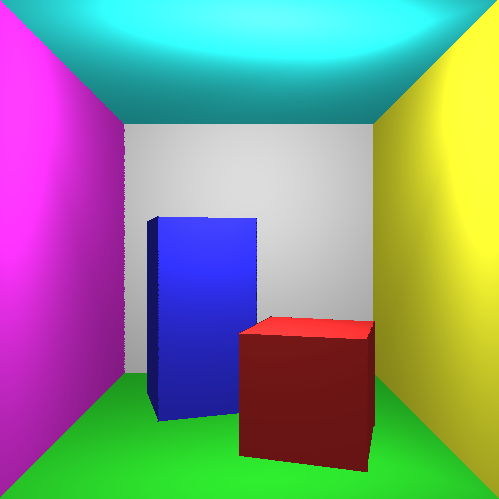
\includegraphics[width=\linewidth]{img/interpolated_pos1.jpg}
\endminipage
\minipage[t]{0.33\textwidth}
    \centering
    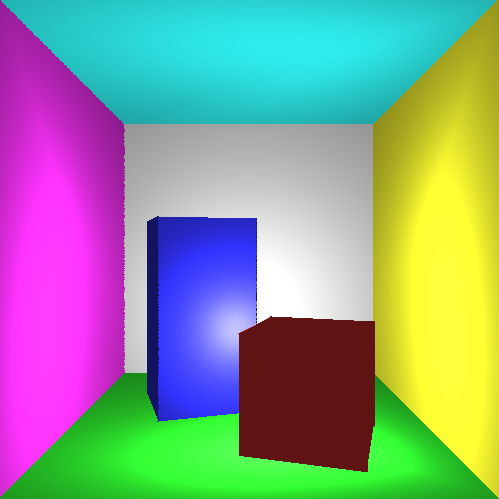
\includegraphics[width=\linewidth]{img/interpolated_pos2.jpg}
\endminipage
\minipage[t]{0.33\textwidth}
    \centering
    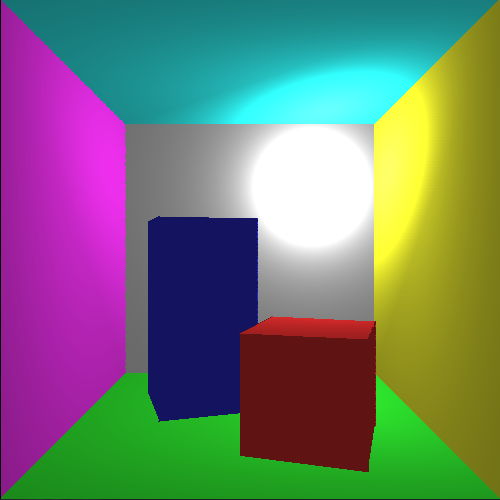
\includegraphics[width=\linewidth]{img/interpolated_pos3.jpg}
\endminipage
\caption{Previous bug sample - Illumination - Interpolated position}
\label{interpolated_pos}
\end{figure}

Those renderings have an inaccurate light surface (figure \ref{interpolated_pos}.1) which may result in unrealistic results (figure \ref{interpolated_pos}.3) when the light moves. The light translation is triggered by the keys W, A, S, D, Q and E.

This is why we must divide the interpolated Z by $\frac{1}{Z}$. The final renderings are computed in 30 ms, while the raytracer gives simlar results (yet including shadows) in 750 ms.

\begin{figure}[H]
\minipage[t]{0.25\textwidth}
    \centering
    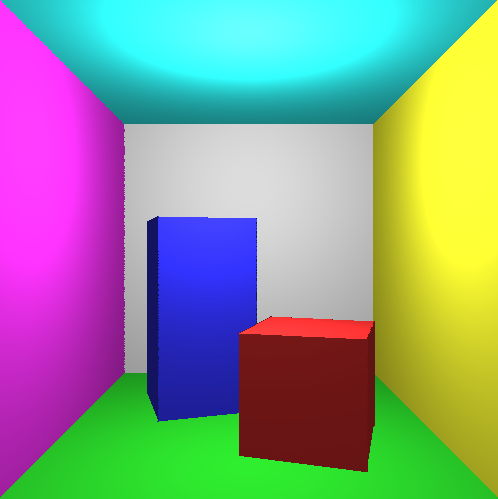
\includegraphics[width=\linewidth]{img/final1.jpg}
\endminipage
\minipage[t]{0.25\textwidth}
    \centering
    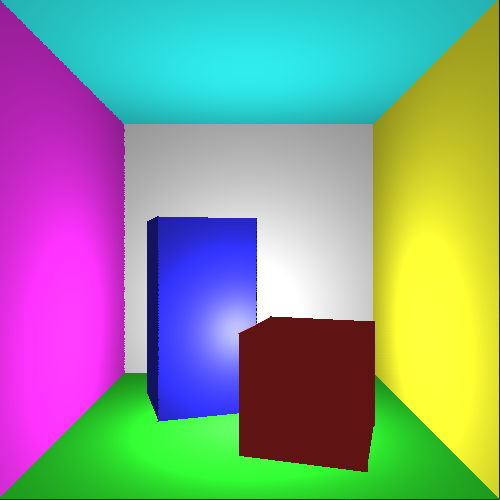
\includegraphics[width=\linewidth]{img/final2.jpg}
\endminipage
\minipage[t]{0.25\textwidth}
    \centering
    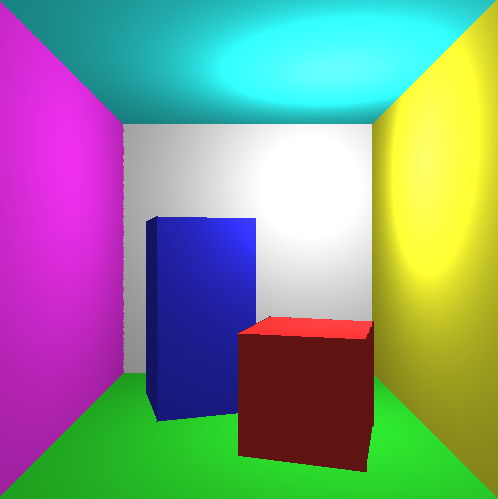
\includegraphics[width=\linewidth]{img/final3.jpg}
\endminipage
\minipage[t]{0.25\textwidth}
    \centering
    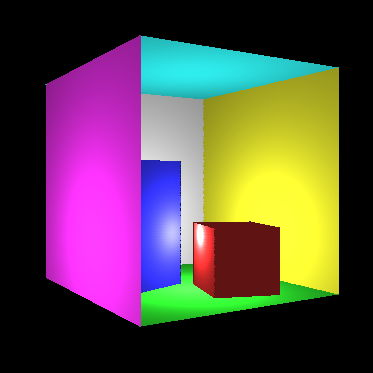
\includegraphics[width=\linewidth]{img/final4.jpg}
\endminipage
\caption{Illumination - Interpolated position}
\end{figure}

